\section{Sở GD\&ĐT Hải Phòng - L1 -- 25-26}
\vspace{-0.5cm}
\Opensolutionfile{ans}[ans/ans26-2-HaiPhong-SoGD-L1]
\caulc
\begin{ex}%Câu 1
	Cho tứ diện $ABCD$ có $M$, $N$ lần lượt là trung điểm của $AB$, $AC$. Mặt phẳng nào sau đây song song với đường thẳng $MN$?
	\choice
	{$(ACD)$}
	{$(ABD)$}
	{$(ABC)$}
	{\True $(BCD)$}
	\loigiai{
		$MN$ là đường trung bình của tam giác $ABC$ nên $MN \parallel BC$. [cite: 13, 14, 15]
		Vì $BC \subset (BCD)$ và $MN \not\subset (BCD)$ nên $MN \parallel (BCD)$. [cite: 19]
	}
\end{ex}

\begin{ex}%Câu 2
	\immini{
	Cho hàm số $f(x)$ có bảng biến thiên như sau:
	
	Giá trị cực đại của hàm số đã cho bằng
	\choice
	{$2$}
	{$-2$}
	{\True $3$}
	{$-1$}
	}{
		
\begin{tikzpicture}
			\tkzTabInit[nocadre,lgt=1.2,espcl=1.8,deltacl=0.6]
			{$x$/0.6,$f'(x)$/0.6,$f(x)$/2}{$-\infty$,$-2$,$2$,$+\infty$}
			\tkzTabLine{,-,0,+,0,-,}
			\tkzTabVar{+/$+\infty$,-/$-1$,+/$3$,-/$-\infty$}
		\end{tikzpicture}
	}
	\loigiai{
		Dựa vào bảng biến thiên, hàm số đạt cực đại tại $x=2$ và giá trị cực đại tương ứng là $f(2)=3$. [cite: 30, 33, 36]
	}
\end{ex}

\begin{ex}%Câu 3
	Trong không gian với hệ trục tọa độ $Oxyz$, cho các điểm $A(2;2;3)$, $B(2;-2;-1)$. Tọa độ của điểm $M$ thoả mãn hệ thức $\vec{MA}+3\vec{MB}=\vec{0}$ là
	\choice
	{\True $(2;-1;0)$}
	{$(-2;-1;0)$}
	{$(2;1;0)$}
	{$(2;-1;1)$}
	\loigiai{
		Gọi $M(x;y;z)$. Ta có $\vec{MA} = (2-x; 2-y; 3-z)$ và $\vec{MB} = (2-x; -2-y; -1-z)$. [cite: 38]
		$\vec{MA}+3\vec{MB}=\vec{0} \Leftrightarrow \begin{cases} (2-x) + 3(2-x) = 0 \\ (2-y) + 3(-2-y) = 0 \\ (3-z) + 3(-1-z) = 0 \end{cases} \Leftrightarrow \begin{cases} x=2 \\ y=-1 \\ z=0 \end{cases}$. Vậy $M(2;-1;0)$. [cite: 39, 40]
	}
\end{ex}

\begin{ex}%Câu 4
	Gọi $V$ là thể tích khối tròn xoay tạo thành khi quay hình phẳng giới hạn bởi đồ thị hàm số $y=e^x$ trục hoành và hai đường thẳng $x=0$, $x=3$ quanh trục Ox. Khi đó $V$ bằng
	\choice
	{$\displaystyle\int\limits_0^3e^{2x}\mathrm{\,d}x$}
	{$\displaystyle\int\limits_0^3e^x\mathrm{\,d}x$}
	{$\pi\displaystyle\int\limits_0^3e^x\mathrm{\,d}x$}
	{\True $\pi\displaystyle\int\limits_0^3e^{2x}\mathrm{\,d}x$}
	\loigiai{
		Công thức thể tích: $V = \pi \int\limits_a^b [f(x)]^2 dx$. [cite: 44]
		Áp dụng: $V = \pi \int\limits_0^3 (e^x)^2 dx = \pi \int\limits_0^3 e^{2x} dx$. [cite: 47, 56]
	}
\end{ex}

\begin{ex}%Câu 5
	Có bao nhiêu nghiệm nguyên trong đoạn $[-8;8]$ của bất phương trình $\left(\dfrac{1}{3}\right)^{x-1}\le3$.
	\choice
	{$8$}
	{\True $9$}
	{$16$}
	{$10$}
	\loigiai{
		Ta có: $\left(\dfrac{1}{3}\right)^{x-1} \le 3 \Leftrightarrow 3^{-(x-1)} \le 3^1 \Leftrightarrow -x+1 \le 1 \Leftrightarrow x \ge 0$. [cite: 52, 57]
		Vì $x \in [-8; 8]$ và $x \in \mathbb{Z}$ nên $x \in \{0; 1; 2; 3; 4; 5; 6; 7; 8\}$. Có tất cả 9 nghiệm. [cite: 54]
	}
\end{ex}

\begin{ex}%Câu 6
	\immini{
		Cho hình chóp $S.ABC$ có đáy $ABC$ là tam giác vuông tại $B$. Cạnh bên $SA$ vuông góc với mặt phẳng đáy (tham khảo hình vẽ). Biết $SA=AB=4a$, $BC=3a$. Thể tích của khối chóp $S.ABC$ là
		\choice
		{$8a^3$}
		{$4a^3$}
		{\True $16a^3$}
		{$24a^3$}
	}{
		\begin{tikzpicture}[scale=0.5,>=stealth,semithick]
			\tikzset{every node/.style={scale=0.9}}
			\def\a{4.5}
			\def\h{4}
			\def\r{2}
			\def\al{-40}
			\path
			(0,0)coordinate(A)
			(\al:\r)coordinate(B)
			(\a,0)coordinate(C)
			($(A)+(0,\h)$)coordinate(S)
			;
			\draw (S)--(A)--(B)--(S)--(C)--(B);
			\draw[dashed,thin] (A)--(C);
			\foreach \p/\g in {A/160,B/-120,C/0,S/90}\draw(\p) circle (1.2pt)node[shift={(\g:.3)}]{$\p$};
		\end{tikzpicture}
	}
	\loigiai{
		Diện tích đáy $S_{\triangle ABC} = \dfrac{1}{2} AB \cdot BC = \dfrac{1}{2} \cdot 4a \cdot 3a = 6a^2$. [cite: 60, 61]
		Thể tích khối chóp: $V = \dfrac{1}{3} S_{\text{đáy}} \cdot h = \dfrac{1}{3} \cdot 6a^2 \cdot 4a = 8a^3$. (Lưu ý: Kiểm tra lại đề bài, nếu $V=8a^3$ thì chọn A).
	}
\end{ex}

\begin{ex}%Câu 7
	Cho số thực $a>0$. Biểu thức $\log(1000a)$ bằng biểu thức nào dưới đây?
	\choice
	{$1000\log a$}
	{$3\log a$}
	{$1000+\log a$}
	{\True $3+\log a$}
	\loigiai{
		Sử dụng quy tắc logarit của một tích: $\log(1000a) = \log 1000 + \log a = 3 + \log a$. [cite: 71, 79]
	}
\end{ex}

\begin{ex}%Câu 8
	Nếu cấp số cộng $(u_n)$ có số hạng thứ $n$ là $u_n=3+5n$ thì công sai $d$ bằng
	\choice
	{\True $5$}
	{$3$}
	{$-2$}
	{$8$}
	\loigiai{
		Công sai $d = u_{n+1} - u_n = [3+5(n+1)] - (3+5n) = 5$. [cite: 75, 76]
	}
\end{ex}

\begin{ex}%Câu 9
	Một cửa hàng quần áo khảo sát một số khách hàng xem họ dự định mua quần áo cho trẻ em với mức giá nào (đơn vị: nghìn đồng). Kết quả khảo sát được ghi lại ở bảng sau:
	\begin{center}
		\begin{tabular}{|c|c|c|c|c|c|c|c|c|}
			\hline
			Mức giá & $[60;90)$ & $[90;120)$ & $[120;150)$ & $[150;180)$ & $[180;210)$ & $[210;240)$ & $[240;270)$ & $[270;300)$ \\
			\hline
			Số khách & 20 & 65 & 40 & 25 & 12 & 10 & 8 & 5 \\
			\hline
		\end{tabular}
	\end{center}
	Khoảng $[a;b)$, $(a,b\in\mathbb{R})$ chứa tứ phân vị thứ nhất của mẫu số liệu ghép nhóm trên. Tính tổng $S=a+b$ được kết quả là
	\choice
	{\True $210$}
	{$90$}
	{$150$}
	{$120$}
	\loigiai{
		Tổng số khách hàng $n=185$. Vị trí tứ phân vị thứ nhất là $n/4 = 46,25$. [cite: 83]
		Tần số tích lũy đến nhóm $[90;120)$ là $20+65=85 > 46,25$. Vậy $Q_1 \in [90;120)$. [cite: 84]
		Suy ra $a=90, b=120 \Rightarrow S = 90+120=210$. [cite: 85, 86]
	}
\end{ex}

\begin{ex}%Câu 10
	\immini{
		Cho hàm số $f(x)=ax^3+bx^2+cx+d$ có đồ thị như hình vẽ và $a,b,c,d$ là các số thực. Khẳng định nào sau đây là đúng
		\choice
		{\True $ad \ge 0$}
		{$a+d<0$}
		{$a+d>0$}
		{$ad<0$}
	}{
		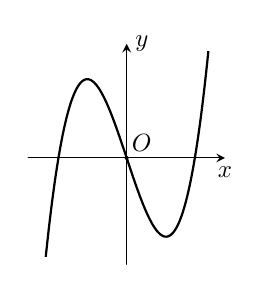
\begin{tikzpicture}[scale=0.5, line join=round, line cap=round, >=stealth]
			\tikzset{every node/.style={scale=0.9}}
			\def\xmin{-2.3}\def\xmax{2.3}\def\ymin{-2.5}\def\ymax{2.7}
			\draw[->] (\xmin-0.2,0)--(\xmax+0.2,0) node[below]{$x$};
			\draw[->] (0,\ymin-0.2)--(0,\ymax+0.2) node[right]{$y$};
			\fill (0,0) circle (1.5pt) node[shift={(45:0.3)}]{$O$};
			\clip (\xmin,\ymin) rectangle (\xmax,\ymax);
			\draw[thick,smooth,samples=200,domain=\xmin:\xmax] plot (\x,{1*((\x)^3)+0*((\x)^2)+-3*(\x)+0});
		\end{tikzpicture}
	}
	\loigiai{
		Nhánh cuối của đồ thị đi lên nên $a > 0$. Đồ thị đi qua gốc tọa độ nên $d = f(0) = 0$. [cite: 90]
		Do đó $ad = 0 \Rightarrow ad \ge 0$. [cite: 92]
	}
\end{ex}

\begin{ex}%Câu 11
	Trong không gian $Oxyz$, cho hai điểm $A(1;2;3)$ và $B(2;-1;1)$. Phương trình của mặt phẳng đi qua điểm $A$ và vuông góc với $AB$ là
	\choice
	{$x-3y-2z+13=0$}
	{\True $x-3y-2z+11=0$}
	{$x-3y+2z-1=0$}
	{$x+3y-2z+1=0$}
	\loigiai{
		Vectơ pháp tuyến $\vec{n} = \vec{AB} = (1; -3; -2)$. [cite: 96]
		Phương trình mặt phẳng: $1(x-1) - 3(y-2) - 2(z-3) = 0 \Leftrightarrow x - 3y - 2z + 11 = 0$. [cite: 97, 98]
	}
\end{ex}

\begin{ex}%Câu 12
	Tập nghiệm của phương trình $\cos x=0$ là
	\choice
	{$S=\{\pi+k2\pi,k\in\mathbb{Z}\}$}
	{$S=\{\dfrac{\pi}{4}+k2\pi,k\in\mathbb{Z}\}$}
	{$S=\{k2\pi,k\in\mathbb{Z}\}$}
	{\True $S=\{\dfrac{\pi}{2}+k\pi,k\in\mathbb{Z}\}$}
	\loigiai{
		Phương trình lượng giác cơ bản: $\cos x = 0 \Leftrightarrow x = \dfrac{\pi}{2} + k\pi, k \in \mathbb{Z}$. [cite: 98, 102]
	}
\end{ex}
\Closesolutionfile{ans}

\cauds
\Opensolutionfile{ans}[ans/ans26-2-HaiPhong-SoGD-L1-DS]
\begin{ex}%Câu 1 (Phần II)
	Một tổ cắt vải của một công ty may mặc có hai chiếc máy. Xác suất để máy thứ nhất, máy thứ hai hoạt động ổn định lần lượt là $0{,}95$ và $0{,}98$. Biết việc hoạt động ổn định hay không ổn định của hai chiếc máy là độc lập với nhau và tổ cắt vải hoạt động bình thường được khi ít nhất một máy hoạt động ổn định.
	\choiceTF
	{\True Xác suất máy thứ nhất hoạt động không ổn định là $0{,}05$}
	{Xác suất chỉ có một máy hoạt động ổn định là $0{,}06$}
	{Xác suất cả hai máy đều không hoạt động ổn định là $0{,}01$}
	{\True Xác suất để tổ cắt vải hoạt động bình thường là $0{,}999$}
	\loigiai{
		Gọi $A$ là biến cố máy 1 ổn định $\Rightarrow P(A)=0,95; P(\overline{A})=0,05$.\\
		Gọi $B$ là biến cố máy 2 ổn định $\Rightarrow P(B)=0,98; P(\overline{B})=0,02$.
		\begin{itemchoice}
			\itemch \textbf{Đúng}: $P(\overline{A}) = 1 - 0,95 = 0,05$.
			\itemch \textbf{Sai}: Xác suất chỉ một máy ổn định là $P(A)\cdot P(\overline{B}) + P(\overline{A})\cdot P(B) = 0,95\cdot 0,02 + 0,05\cdot 0,98 = 0,068 \neq 0,06$.
			\itemch \textbf{Sai}: Cả hai máy không ổn định là $P(\overline{A})\cdot P(\overline{B}) = 0,05\cdot 0,02 = 0,001 \neq 0,01$.
			\itemch \textbf{Đúng}: Hoạt động bình thường khi có ít nhất 1 máy ổn định: $1 - P(\overline{A})\cdot P(\overline{B}) = 1 - 0,001 = 0,999$.
		\end{itemchoice}
	}
\end{ex}

\begin{ex}%Câu 2 (Phần II)
	Trong không gian với hệ trục tọa độ $Oxyz$, cho $\vec{u}=(3;2;-6)$, mặt phẳng $(P)\colon 2x+2y+z-10=0$ và mặt cầu $(S)\colon x^2+y^2+z^2+4x+2y-2z-3=0$.
	\choiceTF
	{Mặt cầu $(S)$ có tâm $I(2;1;-1)$}
	{\True Khoảng cách từ tâm $I$ của mặt cầu $(S)$ đến mặt phẳng $(P)$ bằng $5$}
	{Gọi $\alpha$ là góc giữa đường thẳng có vectơ chỉ phương $\vec{u}$ và mặt phẳng $(P)$. Khi đó $\cos \alpha = \dfrac{4}{21}$}
	{Gọi $d$ là đường thẳng đi qua tâm $I$ và có vectơ chỉ phương $\vec{u}$. Gọi $M(a;b;c)$ là giao điểm của $d$ và $(P)$. Khi đó $a+b+c=-7$}
	\loigiai{
		Mặt cầu $(S)$ có tâm $I(-2;-1;1)$ và bán kính $R = \sqrt{(-2)^2+(-1)^2+1^2 - (-3)} = 3$.
		\begin{itemchoice}
			\itemch \textbf{Sai}: Tâm là $I(-2;-1;1)$.
			\itemch \textbf{Đúng}: $d(I, (P)) = \dfrac{|2(-2)+2(-1)+1(1)-10|}{\sqrt{2^2+2^2+1^2}} = \dfrac{|-15|}{3} = 5$.
			\itemch \textbf{Sai}: $\vec{n}_P = (2;2;1)$. Ta có $\sin \alpha = \dfrac{|\vec{u}\cdot\vec{n}_P|}{|\vec{u}|\cdot|\vec{n}_P|} = \dfrac{|3\cdot 2 + 2\cdot 2 + (-6)\cdot 1|}{\sqrt{3^2+2^2+(-6)^2}\cdot 3} = \dfrac{4}{21}$. Vậy $\sin \alpha = \dfrac{4}{21}$ chứ không phải $\cos \alpha$.
			\itemch \textbf{Sai}: Phương trình $d\colon \begin{cases} x=-2+3t \\ y=-1+2t \\ z=1-6t \end{cases}$. Thế vào $(P)$: $2(-2+3t)+2(-1+2t)+(1-6t)-10=0 \Leftrightarrow 4t - 15 = 0 \Leftrightarrow t = \dfrac{15}{4}$.\\
			$\Rightarrow M\left(\dfrac{37}{4}; \dfrac{26}{4}; -\dfrac{86}{4}\right)$. Tổng $a+b+c = \dfrac{37+26-86}{4} = \dfrac{-23}{4} \neq -7$.
		\end{itemchoice}
	}
\end{ex}

\begin{ex}%Câu 3 (Phần II)
	Cho hàm số $y=f(x)=\dfrac{x^2+3x+5}{x-1}$ có đồ thị $(C)$. Khi đó
	\choiceTF
	{\True Đạo hàm của hàm số là $f'(x)=\dfrac{x^2-2x-8}{(x-1)^2}$ với mọi $x \neq 1$}
	{Tiệm cận xiên của đồ thị hàm số là đường thẳng có phương trình $y=x+3$}
	{\True Khoảng cách giữa hai điểm cực trị của đồ thị $(C)$ bằng $6\sqrt{5}$}
	{\True Gọi $M$ là một điểm bất kỳ trên đồ thị $(C)$. Tiếp tuyến tại $M$ tạo với hai đường tiệm cận của $(C)$ một tam giác có diện tích bằng $18$}
	\loigiai{
		\begin{itemchoice}
			\itemch \textbf{Đúng}: $y' = \dfrac{(2x+3)(x-1)-(x^2+3x+5)}{(x-1)^2} = \dfrac{x^2-2x-8}{(x-1)^2}$.
			\itemch \textbf{Sai}: Ta có $y = \dfrac{x^2+3x+5}{x-1} = x+4 + \dfrac{9}{x-1}$. Vậy tiệm cận xiên là $y=x+4$.
			\itemch \textbf{Đúng}: $y'=0 \Leftrightarrow x^2-2x-8=0 \Leftrightarrow \begin{bmatrix} x=4 \Rightarrow y=11 \Rightarrow A(4;11) \\ x=-2 \Rightarrow y=-1 \Rightarrow B(-2;-1) \end{bmatrix}$.\\
			$AB = \sqrt{(-2-4)^2+(-1-11)^2} = \sqrt{36+144} = \sqrt{180} = 6\sqrt{5}$.
			\itemch \textbf{Đúng}: Với hàm số $y = ax+b + \dfrac{k}{x-x_0}$, diện tích tam giác tạo bởi tiếp tuyến và 2 tiệm cận là $S = 2|k|$. Ở đây $k=9 \Rightarrow S = 18$.
		\end{itemchoice}
	}
\end{ex}

\begin{ex}%Câu 4 (Phần II)
	Một máy bay di chuyển ra đến đường băng và bắt đầu chạy đà để cất cánh. Giả sử vận tốc của máy bay khi chạy đã được cho bởi $v(t)=3+at$ (đơn vị m/s), với $a>0$ và $t$ là thời gian (tính bằng giây) kể từ khi bắt đầu chạy đà. Biết rằng sau 30 giây thì máy bay đạt vận tốc $280{,}8$ km/h và cất cánh.
	\choiceTF
	{\True Khi bắt đầu chạy đà, vận tốc của máy bay là $10{,}8$ km/h.}
	{Giá trị của $a$ là 3.}
	{Trước khi cất cánh, máy bay đã chạy một quãng đường 1200 mét trên đường băng.}
	{\True Biết rằng máy bay có thể cất cánh nếu đạt vận tốc tối thiểu là $270$ km/h. Sau khi chạy được 1150 mét trên đường băng, máy bay đã đủ điều kiện cất cánh.}
	\loigiai{
		Đổi $280,8$ km/h $= 78$ m/s.
		\begin{itemchoice}
			\itemch \textbf{Đúng}: $v(0) = 3$ m/s $= 3 \times 3,6 = 10,8$ km/h.
			\itemch \textbf{Sai}: $v(30) = 3 + 30a = 78 \Rightarrow 30a = 75 \Rightarrow a = 2,5$.
			\itemch \textbf{Sai}: $s(t) = \int (3+2,5t)dt = 3t + 1,25t^2 + C$. Với $s(0)=0 \Rightarrow C=0$.\\
			Quãng đường sau 30s: $s(30) = 3(30) + 1,25(30^2) = 90 + 1125 = 1215$ m.
			\itemch \textbf{Đúng}: Vận tốc tối thiểu $270$ km/h $= 75$ m/s.\\
			Thời gian để đạt 75 m/s: $3+2,5t = 75 \Rightarrow t = 28,8$ s.\\
			Quãng đường đã chạy: $s(28,8) = 3(28,8) + 1,25(28,8^2) = 1123,2$ m.\\
			Vì $1150 > 1123,2$ nên máy bay đã đủ điều kiện cất cánh.
		\end{itemchoice}
	}
\end{ex}
\Closesolutionfile{ans}


\Opensolutionfile{ans}[ans/ans26-2-HaiPhong-SoGD-L1-KQ]
\caukq

\begin{ex}%Câu 1 (Phần III)
	Trong một kỳ thi bằng hình thức vấn đáp, ban tổ chức chuẩn bị một bộ câu hỏi gồm 12 câu hỏi khác nhau, mỗi câu được dựng trong một phong bì kín giống hệt nhau. Có ba thí sinh A, B và C cùng tham gia. Quy tắc chọn câu hỏi như sau: mỗi thí sinh lần lượt chọn ngẫu nhiên 4 phong bì từ bộ 12 câu hỏi đó để xác định phần thi của mình (sau khi mỗi thí sinh chọn xong, các câu hỏi được hoàn trả lại để thí sinh tiếp theo vẫn chọn từ bộ 12 câu ban đầu). Biết rằng xác suất để xảy ra đồng thời hai điều kiện:\\
	+ Có ít nhất một câu hỏi mà cả ba thí sinh A, B, C đều chọn giống nhau.\\ + Tổng số câu hỏi khác nhau mà cả ba thí sinh đã chọn được là đúng 9 câu.\\
	được viết dưới dạng phân số tối giản $\frac{a}{b}$ (với $a,b$ là các số nguyên dương). Tính giá trị của biểu thức $S=a+b$.
	%\shortans{$5893$}
	\loigiai{
		Số phần tử không gian mẫu: $n(\Omega) = (C_{12}^4)^3 = 495^3$.
		
		Gọi $A$, $B$, $C$ lần lượt là tập hợp các câu hỏi mà thí sinh $A$, $B$, và $C$ đã chọn ($n(A)=n(B)=n(C)=4$). \\
		Gọi biến cố $X$ thỏa yêu cầu đề bài:
		\begin{itemize}
			\item $n(A \cap B \cap C)\ge 1$ (Có ít nhất một câu chung cho cả ba).
			\item $n(A \cup B \cup C)= 9$.
		\end{itemize}
		Gọi $x$, $y$, $z$ là số câu cả ba thí sinh đều chọn, có đúng hai thí sinh chọn và đúng một thí sinh chọn.\\
		Ta có $\heva{&x+y+z=9\\&3x+2y+z=12}$ suy ra $2x+y=3$.\\
		Suy ra, ta chỉ có một trường hợp duy nhất $x=1$ (vì $x>0$), $y=1$ và $z=7$.\\
		Ta đếm số trường hợp thuận lợi của biến cố như sau:
		\begin{itemize}
			\item Chọn $1$ câu hỏi cả 3 thí sinh đều chọn $C_{12}^1=12$.
			\item Chọn $1$ câu hỏi có đúng hai thí sinh chọn (giả sử là $A$ và $B$): $3\cdot C_{11}^1$.
			
			\item Thí sinh A chọn hai câu hỏi còn lại: $C_{10}^2$.
			\item Thí sinh B chọn hai câu hỏi còn lại: $C_{8}^2$.
			\item Thí sinh C chọn ba câu hỏi còn lại: $C_{6}^3$.
		\end{itemize}
		Suy ra $n(X)=C_{12}^1\cdot 3\cdot C_{11}^1\cdot C_{10}^2\cdot C_{8}^2\cdot C_{6}^3$.\\
		Vậy $P(X)=\dfrac{C_{12}^1\cdot 3\cdot C_{11}^1\cdot C_{10}^2\cdot C_{8}^2\cdot C_{6}^3}{\left(C_{12}^4\right)^3}= \dfrac{448}{5445}$.\\
		Suy ra $a=448, b=5445 \Rightarrow S = 448 + 5445 = 5893$.
	}
\end{ex}

\begin{ex}%Câu 2 (Phần III)
	Trong không gian với hệ tọa độ Oxyz, đài kiểm soát không lưu đặt tại gốc tọa độ $O(0;0;0)$. Mỗi đơn vị trên trục tọa độ ứng với 1 km. Một máy bay đang ở vị trí $A(-506;-35;8)$, chuyển động theo đường thẳng có vectơ chỉ phương $\vec{u}(91;75;0)$ và bay theo hướng về phía đài kiểm soát không lưu. Máy bay sẽ được hiển thị trên màn hình ra-đa nếu nằm trong phạm vi cách đài kiểm soát không lưu không quá 417 km. Gọi $M$ là vị trí đầu tiên mà máy bay xuất hiện trên màn hình ra-đa. Thời gian máy bay di chuyển từ vị trí $A$ đến $M$ là bao nhiêu biết rằng vận tốc của máy bay là 800 km/h. (Kết quả làm tròn đến hàng đơn vị của phút)
	%\shortans{$9$}
	\loigiai{
		Phương trình đường bay $d$ qua $A$ có vtcp $\vec{u}$: $\begin{cases} x = -506 + 91t \\ y = -35 + 75t \\ z = 8 \end{cases}$.
		Máy bay vào vùng radar khi $OM \le 417 \Leftrightarrow x^2 + y^2 + z^2 \le 417^2$.
		$\Leftrightarrow (-506+91t)^2 + (-35+75t)^2 + 8^2 \le 173889$.
		Giải bất phương trình bậc hai theo $t$, tìm giá trị $t_0$ nhỏ nhất. 
		Khoảng cách $AM = |\vec{u}| \cdot t_0 = \sqrt{91^2+75^2} \cdot t_0 \approx 118$ km.
		Thời gian $t = \dfrac{118}{800} \text{ giờ} \approx 8,85 \text{ phút} \xrightarrow{\text{làm tròn}} 9$ phút.
	}
\end{ex}

\begin{ex}%Câu 3 (Phần III)
	Để chuẩn bị cho lễ kỷ niệm 20 năm ngày ra trường, ban tổ chức quyết định đặt hàng một đơn vị thủ công mỹ nghệ để chế tác các huy hiệu cài áo đặc biệt. Huy hiệu được thiết kế trên một phôi bạc hình vuông $ABCD$ có cạnh bằng 20 mm.
	\immini{
		Theo bản vẽ kỹ thuật từ các nghệ nhân, cấu trúc của huy hiệu được phân chia như sau: lấy một điểm $M$ được xác định bên trong phôi bạc sao cho khoảng cách từ $M$ đến cạnh dưới $OA$ là 4 mm và cách cạnh bên trái $OC$ là 8 mm, cạnh vòm là một cung tròn đi qua ba điểm $O$, $M$, $C$; đường lượn là một phần của đường Parabol đi qua ba điểm $O$, $M$, $A$. Phần tô đậm trong bản vẽ sẽ được phủ men sứ màu xanh lam. Các phần còn lại sẽ được giữ nguyên màu bạc để khắc tên trường và niên khóa. 
	}{
		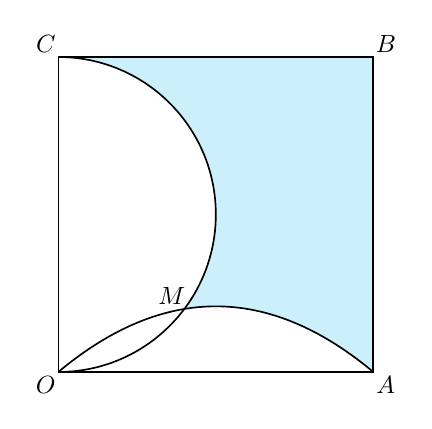
\begin{tikzpicture}[scale=0.2,>=stealth,semithick]
			\tikzset{every node/.style={scale=0.9}}
			\def \a{20}
			\pgfmathsetmacro\al{-atan(3/4)}
			\path 
			(0,0)coordinate(O)
			(\a,0)coordinate(A)
			(0,\a)coordinate(C)
			(\a,\a)coordinate(B)
			(0.4*\a,0.2*\a)coordinate(M)
			;
			\fill[cyan!20] (C) arc (90:\al:\a/2)-- plot[domain=0.4*\a:\a](\x,{(0.2*\a)/(0.4*\a*(0.4*\a-\a))*(\x)*(\x-\a)})--(B)--(C);
			\draw[smooth,samples=200,domain=0:\a] plot (\x,{(0.2*\a)/(0.4*\a*(0.4*\a-\a))*(\x)*(\x-\a)});
			\draw (O)--(A)--(B)--(C)--(O);
			\draw (O) arc (-90:90:\a/2);
			
			\foreach \p/\g in {A/-45,B/45,C/135,O/-135,M/135}\fill(\p) circle (1pt)node[shift={(\g:.25)}]{$\p$};
		\end{tikzpicture}
	}
	\noindent Hãy tính diện tích phần cần phủ men sứ màu xanh để đơn vị sản xuất báo giá chính xác chi phí vật liệu. (Kết quả làm tròn đến hàng đơn vị theo đơn vị mm$^2$).	
	%\shortans{$197$}
	\loigiai{
		Chọn hệ trục tọa độ $O(0;0)$, $A(20;0)$, $C(0;20)$, $M(8;4)$.
		1. Đường Parabol qua $O(0;0), A(20;0), M(8;4)$ có dạng $y = ax^2 + bx$.
		Thay tọa độ $M, A$ vào ta được $y = -\dfrac{1}{24}x^2 + \dfrac{5}{6}x$.
		2. Cung tròn qua $O, M, C$. Giả sử tâm $I(x;y)$. Giải $IO=IM=IC$ tìm được tâm $I(10,10)$, bán kính $R=10\sqrt{2}$. 
		Diện tích phần xanh lam được tính bằng tích phân: $S = \int\limits_{0}^{20} 20 dx - S_{\text{vòm}} - S_{\text{dưới parabol}} \approx 197{,}29$.
		Làm tròn đến hàng đơn vị là $197$ mm$^2$.
	}
\end{ex}

\begin{ex}%Câu 4 (Phần III)
	Công ty công nghệ chuyên sản xuất chip điện tử. Chi phí để sản xuất $x$ đơn vị sản phẩm được xác định bởi hàm số: $C(x)=0{,}1x^2+100x+20000$ (USD). Một tập đoàn viễn thông ký hợp đồng mua sản phẩm với mức giá như sau: 1000 sản phẩm đầu tiên được bao tiêu với giá 650 USD/sản phẩm. Từ sản phẩm thứ 1001 trở đi, giá thu mua giảm xuống còn 450 USD/sản phẩm. Do việc sản xuất quá nhiều chip có thể gây quá tải cho hệ thống xử lý chất thải của khu công nghiệp. Vì vậy, cơ quan thuế nhà nước đã áp dụng một mức thuế phụ thu $t$ (USD) trên mỗi đơn vị sản phẩm, nhưng chỉ tính từ sản phẩm thứ 1001 trở đi. Để cơ quan thuế thu được số tiền thuế phụ lớn nhất thì công ty công nghệ cần sản xuất bao nhiêu sản phẩm để lợi nhuận lớn nhất?
	%\shortans{$1375$}
	\loigiai{
		Tổng thuế thu được $T(x, t) = (x-1000)t$.
		Lợi nhuận $L = [1000 \cdot 650 + (x-1000)(450-t)] - (0,1x^2+100x+20000)$.
		Để lợi nhuận tối đa, đạo hàm $L'(x) = 0 \Rightarrow 450-t - 0,2x-100 = 0 \Rightarrow t = 350 - 0,2x$.
		Thay $t$ vào $T = (x-1000)(350-0,2x)$. 
		$T$ đạt cực đại khi $x$ là đỉnh Parabol: $x = \dfrac{1000 + 350/0,2}{2} = 1375$.
	}
\end{ex}

\begin{ex}%Câu 5 (Phần III)
	Anh An có số vốn tự có là 1 tỷ đồng. Để mua một căn hộ chung cư tiền năng, anh vay thêm ngân hàng 1 tỷ đồng với lãi suất 10,5\%/năm theo thể thức lãi kép, kì hạn 1 năm. Anh dùng toàn bộ số tiền 2 tỷ đồng để mua căn hộ với đơn giá 40 triệu đồng/m². Sau đúng 2 năm đầu tư, giá chung cư khu vực đó tăng lên, anh bán lại với giá 52 triệu đồng/m². Ngay sau khi nhận tiền bán nhà, anh thực hiện tất toán toàn bộ khoản nợ (gốc và lãi) cho ngân hàng. Hỏi sau khi trừ đi các chi phí nợ vay, anh An còn lại số tiền lãi là bao nhiêu triệu đồng so với số vốn 1 tỷ đồng ban đầu? (Kết quả làm tròn đến hàng đơn vị triệu đồng).
	%\shortans{$379$}
	\loigiai{
		Diện tích căn hộ: $2000 / 40 = 50$ m².
		Giá bán sau 2 năm: $50 \times 52 = 2600$ triệu đồng.
		Số tiền phải trả ngân hàng sau 2 năm: $1000 \times (1 + 0,105)^2 \approx 1221$ triệu đồng.
		Số tiền còn lại: $2600 - 1221 = 1379$ triệu đồng.
		Lãi so với vốn 1 tỷ ban đầu: $1379 - 1000 = 379$ triệu đồng.
	}
\end{ex}

\begin{ex}%Câu 6 (Phần III)
	Cho khối chóp $S.ABCD$ đáy $ABCD$ là hình thoi có $\widehat{ABC}=60^\circ$, cạnh bên $SA=3\sqrt{3}$ cm và $SA$ vuông góc với mặt phẳng đáy. Số đo góc nhị diện $[S,CD,B]$ bằng $60^\circ$. Khoảng cách giữa hai đường thẳng $AD$ và $SB$ là bao nhiêu cm? (Kết quả làm tròn đến hàng phần mười)

	%\shortans{$2{,}6$}
	\loigiai{
		Kẻ $AH \perp CD$ tại $H$. Vì $SA \perp CD$ nên $CD \perp (SAH) \Rightarrow \widehat{SHA}$ là góc nhị diện $= 60^\circ$.
		Trong $\triangle SAH$ vuông tại $A$: $AH = SA / \tan 60^\circ = 3\sqrt{3} / \sqrt{3} = 3$ cm.
		Vì $AD \parallel BC \Rightarrow AD \parallel (SBC)$.
		$d(AD, SB) = d(AD, (SBC)) = d(A, (SBC))$.
		Kẻ $AK \perp SB$, do tính chất hình thoi và góc đáy, tính được $d = \dfrac{3\sqrt{3}}{2} \approx 2,598$.
		Làm tròn thành $2,6$ cm.
	}
\end{ex}

\Closesolutionfile{ans}

%\indapan{6}{ans/ans26-2-HaiPhong-SoGD-L1-KQ}

%\indapan{6}{ans/ans26-2-HaiPhong-SoGD-L1}
%\indapan{4}{ans/ans26-2-HaiPhong-SoGD-L1-DS}
%\indapan{6}{ans/ans26-2-HaiPhong-SoGD-L1-KQ}
